\documentclass{article}

% Imports
\usepackage{graphicx} % Required for inserting images
\usepackage{geometry}[left=1cm, right=1cm]
\usepackage{amsfonts, amsmath, amssymb, amsthm}
\usepackage{xcolor}
\usepackage{biblatex}
\usepackage{hyperref}
\usepackage{thmtools, mdframed}

\newcounter{question}[section]
\newenvironment{question}[1][]{\refstepcounter{question}\par 
   \noindent \textbf{Question \thequestion #1.} \medskip}{\medskip}

\newcounter{answer}[section]
\newenvironment{answer}[1][]{\refstepcounter{answer}\par
   \noindent\textbf{Answer \theanswer #1.} \medskip }{\medskip $\triangle$}

\newcommand{\E}{\mathbb{E}}
   


\title{Senior Thesis Notes}
\author{Spencer Venancio}
\date{}

\addbibresource{ref.bib}

\begin{document}

\maketitle

\section{04-01-2026 Meeting}
\begin{itemize}
    \item Can we devise a model agnostic approach to handle correlated features?
    \item Can we adapt LOCO or MinShap?
    \item Example to keep in mind: the MNIST dataset---each individual pixel isn't useful, but patches are. So how big of a patch do we need?
    \item How do we want to represent the importance of each pixel?
    \item Start with image or spatial data, explore some form of feature selection or cluster selection.
\end{itemize}

With LOCO we have an example with correlated features where none of the features are selected (compared to LASSO, where a single representative is chosen). In the LASSO case, it's not clear that we would select the ``right'' representative, or that selecting a single representative is even the right thing to be looking for. From a qualitative perspective we might want to keep all of the features within a correlated cluster. We can look at the GTV paper as an example of this---although not model agnostic---where they use the idea of alignment to evenly spread coefficient weight across the cluster. We would like to do something similar in a model agnostic setting, perhaps by adapting LOCO or MinShap.

{\color{red} \textbf{TODO:}
\begin{itemize}
    \item Look into the MNIST dataset. Explore the effects of patch size on wrapper method feature selection methods (LOCO, MinShap, etc.).
    \item Think about how to enforce alignment in these wrapper methods.
    \item Try to formalize a specific research problem.
\end{itemize}}

\subsection{Notes}

\subsubsection{MinShap Paper}
Shapley values are a widely used method in machine learning for feature importance. We can view them as a wrapper method, as they can be used regardless of the predictive model. The issue is that nonzero Shapley values do not imply nonzero feature importance.

We can modify the approach for feature selection: instead of averaging over $K$ feature permutations, we take the minimum over $K$. This works because there will always exist some ordering where $X_j$ is placed after all of the features that ``explain away'' its contribution.

\textbf{Assumptions.}
\begin{enumerate}
    \item \emph{Faithfulness.} All of the independence relationships are exactly caused by the graph. I.e. there are no cancellations.
    \item \emph{No data leakage / reverse causation.} There is no causal path from $Y$ to any of the features $X_j$.
\end{enumerate}

\subsubsection{GTV Paper}
Standard regularization methods like LASSO work under the assumption of independence of features, or under mild dependence assumptions. But this is often not the case in practice, and the lack of independence leads to undetermined solutions $\beta^*$.

This is expressed by the situation when $\lambda_i(\Sigma) = 0$, or $\lambda_i(\Sigma) \approx 0$, which represents the case where very large perturbations in the data can lead to practically the same result.

The paper proposes a solution to this problem via an additional assumption of \emph{alignment}.

\textbf{Assumptions.}
\begin{enumerate}
    \item \emph{Alignment.} The coefficients of $\beta^*$ for correlated features $X_j, X_k$ are similar and match in direction.
    \item There is a finite $\max_i \lambda_i(\Sigma)$.
    \item The $\ell_1$ norm for each row/column is lower bounded by a constant.
    \item We have a sufficiently good estimator $\hat \Sigma$ for $\Sigma$.
\end{enumerate}

Interestingly, our estimator $\hat \Sigma$ doesn't need to rely on $X$---we can instead rely on side information.

\section{04-23-2026 Meeting}
After exploring LOCO and MinShap for various patch sizes using log-loss and accuracy as the loss function, we want to explore others. In particular we would like to explore a local measure
\[ 
    V(S) =\mathbb E[f(X) | X_S = x_S].
\]
In order to calculate this quantity in practice can use a $k$-nearest neighbors approach. I.e. 
\[ 
    \frac 1 n \sum_{j=1}^n f(X_{-S}^{(j)} , X_{S}^{(i)}).
\]
The reason for doing so would be to get a local version of MinShap, which would give us a \emph{local feature selection method}. 
{\color{red} \textbf{TODO:}
\begin{itemize}
    \item Implement the local loss function for MinShap.
    \item Experiment with the loss function on the MNIST data set.
\end{itemize}}

\subsection{Notes}
To get a better understanding of \textbf{local feature selection} I read the introduction of \cite{gimenez2019discoveringconditionallysalientfeatures}. To think about its usefulness it's helpful to think about a genomics example. Consider the situations where $A$ is associated with the desired phenotype across the whole dataset, but conditioned on $B$ being present $Y$ is independent of $A.$ $A$ is therefore globally important, but not locally when in a certain area of the feature space.
\begin{question}
    What is the difference between local feature attribution and selection? 
\end{question}
\begin{answer}
    Feature attribution aims to give a post-hoc measure of how each feature in a model contributed to a model prediction, Ex. Shapely Values or $\beta_i X_i$. This will give us a ranking of features. Whereas with local feature selection we get a subset of features, with statistical guarantees. {\color{blue} What's still unclear to me is whether we get different prediction functions under this regime.}
\end{answer}
\begin{question}
    What is the purpose of local feature selection?
\end{question}
\begin{answer}
    It seems to me that local feature selection is more about understanding complex interactions between features and outcomes as in the genomics exampl rather than to select a feature set to actually train a predictive model.
\end{answer}

The proposed value function will look something like 
\[ 
\E [f(X) |X_S = x_S] \sim \E [f(\underbrace{x_1, x_2, \dots , x_{k-1}}_\text{fixed values ($S$)}, \underbrace{X_k, X_{k+1}, \dots,X_n}_\text{random variables})]
\]
So the idea for computing this is that you fix an image $x^*=(x_1, \dots, x_p)\in X.$ Then for the different subset $S$ in the Shapely value computations you have a set of indices which are fixed. Then the $K$-nearest neighbors approach comes from setting a tolerance $\alpha$. Then you take a average of the prediction function over the $x\in X$ such that $|x_i|\le \alpha$ for all $i \in S.$ 

I have some uncertainties about using this function in MinShap:

{\color{blue}
\begin{itemize}
    \item This function isn't a loss function, it measures how much much prediction changes. So it's not clear to me that we can use this function for feature importance or feature selection vs. feature attribution. 
    \item It appears that the function $f$ doesn't use retraining. This feels like a big departure from the way that MinShap works. 
\end{itemize}
}

From line 8 Algorithm 1 from the MinShap paper: 

{ \centering Fit model $f_{n,\mathcal{P}_{j-1}^{\pi_k} \cup \{j\}}$ and compute $V_{\text{new}} \leftarrow V(f_{n,\mathcal{P}_{j-1}^{\pi_k} \cup \{j\}}, P_n)$ \par}

This retraining isn't occurring at all with the proposed function. I think we need to incorporate some retraining. What if we instead did something like 
\[ 
\E[(Y- f_S(X))^2|X_S=x_S]
\]

\section{04-30-2026 Meeting}
Local feature selection methods are indeed more about analysis than determining the ideal feature set for a predictive model, eg. genomics phenotype examples. We would likely only run this local feature selection method on a singular or small set of examples, not the whole set. {\color{red} \textbf{TODO:}
\begin{itemize} 
    \item Implement the $\E[(Y- f_S(X))^2|X_S=x_S]$ value function for MinShap
    \item We can also explore credit loan approval datasets
    \item We might also look into the situation where the digit we are trying to predict is entirely absent from the training set. 
    \begin{itemize}
        \item You wouldn't predict the correct digit, but the feature selections could still be interesting
    \end{itemize}
\end{itemize}}
\subsection{Notes}
T
Our proposed value function $\E[(Y-f_S(X))^2 |X_S = x_S]$ has an issue because of non-monotonicity. MinShap relies on the value function being monotonic: i.e. the model always gets better when you add more features. This is true globally, but it's very well possible that adding a feature doesn't improve predictions for a specific example. 

\section{05-08-2026 Meeting}
\begin{itemize}
    \item Look into saliency maps
    \begin{itemize}
        \item calculate some saliency maps
        \item if a gradient is small, what does that mean
    \end{itemize}
    \item Go back to the basics of feature selection, we tried the purely experimental approach, but now we need to figure out how much of the ideas from global FS carry over
    \item Touch base after I get back
\end{itemize}

\textbf{ We have two open questions: }
\begin{enumerate}\color{blue}
    \item How to determine the threshold for selection (statistical question)

    \item For integrated gradients, can we replace the integral operator with a min(.) operator to get a good feature selection method
\end{enumerate}

\textbf{\color{red} TODO:} use simple image data, and generate saliency maps and integrated gradients and see how they look.

\subsection{Notes}
Saliency maps and integrated gradients exist together, and integrated gradients seek to solve a problem created by saliency maps. The natural progression is saliency maps (vanilla gradients) $\rightarrow$ inputs$\times$gradients $\rightarrow$ integrated gradients. All of these methods require the assumption to be differentiable, so it works for neural networks (most common application) and regression, but breaks down on tree based methods. 

\subsubsection{Saliency Maps}


The basic idea of saliency is 
\[ 
\mathrm{saliency} = \frac{\partial \mathrm {output}}{\partial \mathrm {input}}.
\]
Thus it can provide us with a way of identifying key pixels/patches. The most basic version of saliency maps is \emph{vanilla gradients.} Given a pretrained model $f$ and an image $\mathbf x= x_1, x_2, \dots, x_n$ the saliency for a pixel $i$ is
\[ 
S_i =  \frac{\partial f(\mathbf x)}{\partial x_i}.
\]
In the classification context we can be a little more precise and say that for a $K$-class classifier, where $c\in \{1, 2, \dots, K \}$ is the class of the local image $\mathbf x$  then the saliency is 
\[ 
S_i =  \frac{\partial f_c(\mathbf x)}{\partial x_i},
\]
where $f_c$ is the logit or softmax probability for class $c.$

\begin{figure}[!htb]
    \centering
    \begin{minipage}{.3\textwidth}
        \centering
        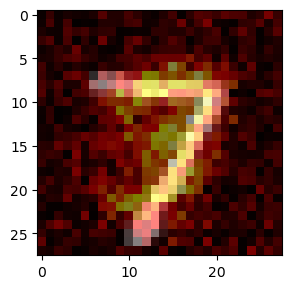
\includegraphics[width=0.7\linewidth]{img/saliency_map_0.png}
    \end{minipage}%
    \begin{minipage}{0.3\textwidth}
        \centering
        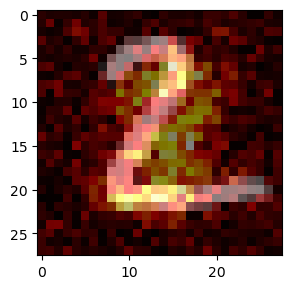
\includegraphics[width=0.7
        \linewidth]{img/saliency_map_1.png}
        \label{fig:prob1_6_1}
    \end{minipage}
    \begin{minipage}{0.3\textwidth}
        \centering
        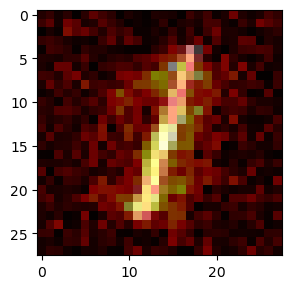
\includegraphics[width=0.7
        \linewidth]{img/saliency_map_2.png}
        \label{fig:prob1_6_1}
    \end{minipage}
    \caption{Saliency Maps for the MNIST DATA}
\end{figure}

\subsubsection{Integrated Gradients}
There is an issue with saliency maps where a pixel/feature has a high gradient, but the feature value (input) is 0--the feature is no different from the baseline. With vanilla gradients, we would represent the feature as important because the gradient is high, but this would be misleading, because the feature isn't contribution to prediction if that feature isn't moving from the baseline. This motivates the method of inputs$\times$gradients, because in this case, given a large gradient $d$ and an input of $0$ we observe an attribution of $0d=0.$

We can actually see the method of inputs$\times$gradients as a special case of computing integrated gradients in practice. The formula for integrated gradients is 
\[ 
    IG_i(\mathbf x) = (\mathbf x - \mathbf x_0)\int_0^1 \frac{\partial f_c (\mathbf x_0 + \alpha(\mathbf x - \mathbf x_0))}{\partial x_i} d\alpha.
\]
Which, in practice we compute as 
\[ 
    \widehat{IG}_i(\mathbf x) = (\mathbf x - \mathbf x_0) \cdot \frac 1 m \sum_{k=1}^m \frac{\partial f_c(\mathbf x_0 + \frac km(\mathbf x - \mathbf x_0))}{\partial x_i}.
\]
Where $m$ is the number of steps along the path, and we can see that inputs$\times$gradients is the case when $m=1.$ 

The advantage that integrated gradients has is the opposite problem, when we have a near 0 gradient, because the model is confident in it's prediction, such that individual pixels can't really affect model prediction. This problem is solved by following a path, and computing the gradient at each step, where the path is from say a black image to the full input image. It's the information from the earlier parts of the path that will demonstrate that certain pixels are more important than just what we'd see from inputs$\times$gradients.

\begin{figure}[!htb]
    \centering
    \begin{minipage}{.3\textwidth}
        \centering
        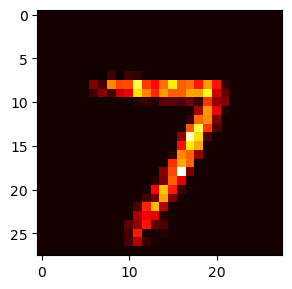
\includegraphics[width=0.7\linewidth]{img/input_x_gradient_0.png}
    \end{minipage}%
    \begin{minipage}{0.3\textwidth}
        \centering
        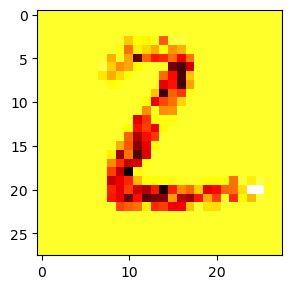
\includegraphics[width=0.7
        \linewidth]{img/input_x_gradient_1.png}
        \label{fig:prob1_6_1}
    \end{minipage}
    \begin{minipage}{0.3\textwidth}
        \centering
        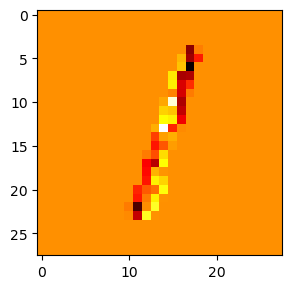
\includegraphics[width=0.7
        \linewidth]{img/input_x_gradient_2.png}
        \label{fig:prob1_6_1}
    \end{minipage}
    \caption{Inputs $\times$ Gradients for the MNIST DATA}
        \centering
    \begin{minipage}{.3\textwidth}
        \centering
        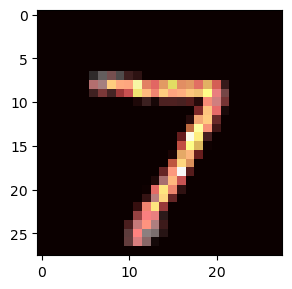
\includegraphics[width=0.7\linewidth]{img/integrated_gradients_0.png}
    \end{minipage}%
    \begin{minipage}{0.3\textwidth}
        \centering
        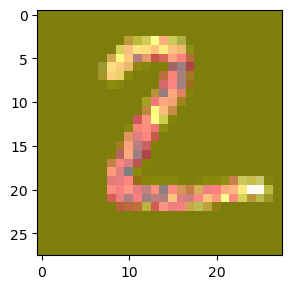
\includegraphics[width=0.7
        \linewidth]{img/integrated_gradients_1.png}
        \label{fig:prob1_6_1}
    \end{minipage}
    \begin{minipage}{0.3\textwidth}
        \centering
        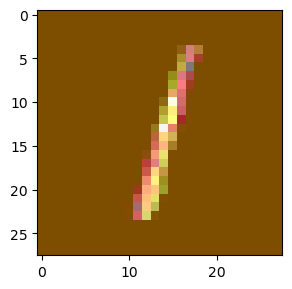
\includegraphics[width=0.7
        \linewidth]{img/integrated_gradients_2.png}
        \label{fig:prob1_6_1}
    \end{minipage}
    \caption{Integrated Gradients for the MNIST DATA}
\end{figure}

\section{06-04-2026 Meeting}

\begin{itemize}
    \item Look at a mixture of both simulated and real dataset 
    \begin{itemize}
        \item MinShap paper as an example 
        \item Class examples. Ex. XOr
    \end{itemize}
    \item Look back into adapting MinShap with new $VI_j^S$
    
\end{itemize}


generalized covariance measure--gcm

\end{document}
